\documentclass{jsarticle}
\usepackage[dvipdfmx]{graphicx}
\usepackage{listings}
\usepackage{afterpage}
\begin{document}
\title{課題2 色階調変化}
\author{13EC060 武澤 裕介}
\maketitle
\begin{abstract}
まずmatlabを用いて画像の色階調を変化させる、また今回課題で用いたプログラムをpythonに書き換えたものも付録として掲載する。
\end{abstract}
\section{色階調の変化}
まず、今回使用する原画像を図1に示す。
\begin{lstlisting}[basicstyle=\ttfamily\footnotesize, frame=single]
filename = uigetfile('*');
ORG=imread(filename); % 原画像の入力
ORG = rgb2gray(ORG); colormap(gray); colorbar;
imagesc(ORG); axis image; % 画像の表示
pause; % 一時停止
 \end{lstlisting}
を用いてまず入力画像のグレースケール画像を表示させる。

\begin{figure}[htbp]
 \begin{center}
  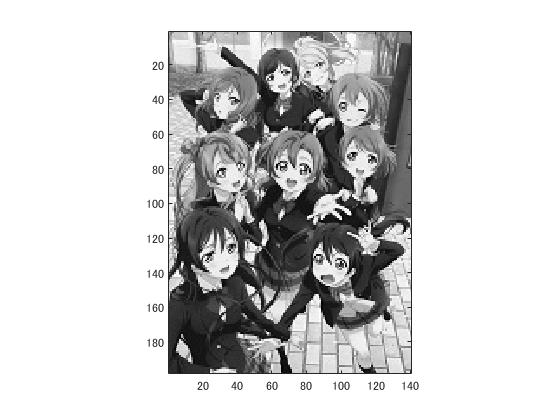
\includegraphics[width=10cm]{kadai2-0.jpg}
 \end{center}
 \caption{原画像}
\end{figure}

次に2色階調画像を作成する。最大輝度値に対して半分の輝度値をしきい値として扱い画像を変換すればよい。つまり
\begin{lstlisting}[basicstyle=\ttfamily\footnotesize, frame=single]
IMG = ORG>128;
 \end{lstlisting}
としきい値を設定する。

\begin{figure}[htbp]
 \begin{center}
  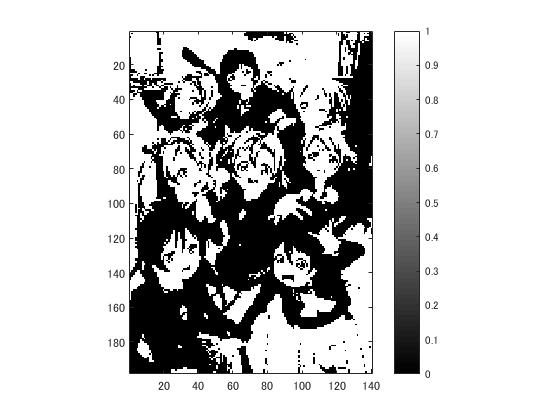
\includegraphics[width=10cm]{kadai2-1.jpg}
 \end{center}
 \caption{2色階調画像}
\end{figure}

次に4色階調画像を作成する。最大輝度値に対して1/4、1/2、3/4の輝度値をしきい値として扱い画像を変換すればよい。つまり
\begin{lstlisting}[basicstyle=\ttfamily\footnotesize, frame=single]
IMG0 = ORG>64;
IMG1 = ORG>128;
IMG2 = ORG>192;
IMG = IMG0 + IMG1 + IMG2;
\end{lstlisting}
としきい値を設定する。

\newpage

\begin{figure}[htbp]
 \begin{center}
  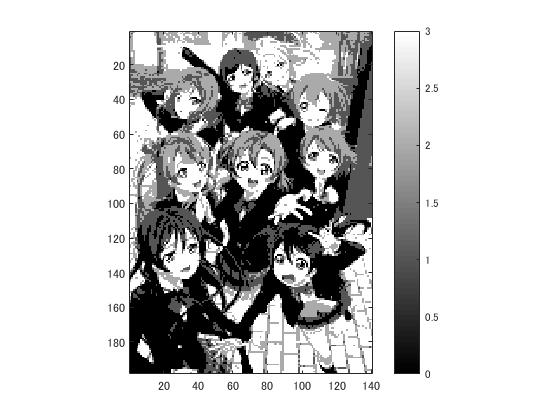
\includegraphics[width=10cm]{kadai2-2.jpg}
 \end{center}
 \caption{4色階調画像}
\end{figure}


次に8色階調画像を作成する。最大輝度値に対して1/8、1/4、3/8、1/2、5/8、3/4の輝度値をしきい値として扱い画像を変換すればよい。つまり
\begin{lstlisting}[basicstyle=\ttfamily\footnotesize, frame=single]
IMG0 = ORG>32;
IMG1 = ORG>64;
IMG2 = ORG>96;
IMG3 = ORG>128;
IMG4 = ORG>160;
IMG5 = ORG>192;
IMG6 = ORG>224;
IMG = IMG0 + IMG1 + IMG2 + IMG3 + IMG4 +IMG5 + IMG6;
\end{lstlisting}
としきい値を設定する。
\newpage
\begin{figure}[htbp]
 \begin{center}
  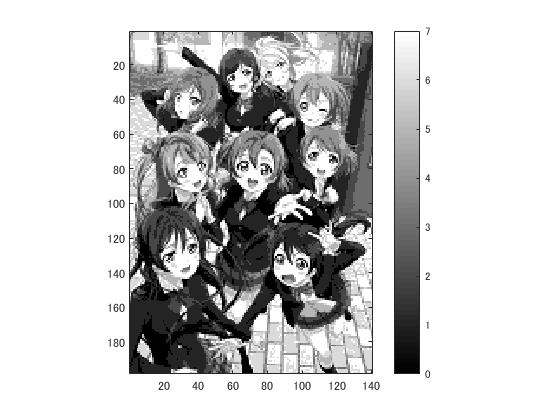
\includegraphics[width=10cm]{kadai2-3.jpg}
 \end{center}
 \caption{8色階調画像}
\end{figure}

\section{考察}
今回色階調の変化による画像の変化を観察する事によって色階調を減らす事により疑似輪郭の発生を観測することができた。特に図2、図3において疑似輪郭は確かに観測できる。ただ、図4の8色階調画像においては特に疑似輪郭は観測できなく、原画像とほぼ同一な画像であり画素の欠損が少ないと言える。
\newpage
\section{付録-python2.x系列による色階調変更コード-}
\begin{lstlisting}[basicstyle=\ttfamily\footnotesize, frame=single]
#-*-coding:utf-8-*-
import cv2
import numpy as np
import sys  
  
argvs=sys.argv  
if (len(argvs) != 2):  
 print 'Usage: # python %s filename' % argvs[0]  
 quit()   
            
imagefilename = argvs[1]  
try:  
 img=cv2.imread(imagefilename, 1)  
except:  
 print 'faild to load %s' % imagefilename  
 quit()    

img = cv2.cvtColor(img,cv2.COLOR_BGR2GRAY)
gradationNum = input('何階調にしますか?')
width = img.shape[0]
height = img.shape[1]
temp = np.zeros_like(img)
for i in range(1,gradationNum):
 for j in xrange(width):
  for k in xrange(height):
   if img[j,k]>(256/gradationNum)*i: 
    temp[j,k] += (256/gradationNum)*i
GraditionName = raw_input('please fileName after GraditionTransformation') 
cv2.imwrite(GraditionName,temp)
\end{lstlisting}
\end{document}